\section{Diagrammi di attività}
In seguito vengono descritte le interazioni dell'utente con MaaS. Per fare questo sono utilizzati i diagrammi di attività, esposti seguendo la struttura presente nell'analisi dei requisiti:
\begin{itemize}
\item \textbf{Utente non autenticato};
\item \textbf{Utente autenticato};
\item \textbf{Editor};
\item \textbf{Super admin}.
\end{itemize}
\subsection{Utente non autenticato}
\begin{figure}[H]
\begin{center}
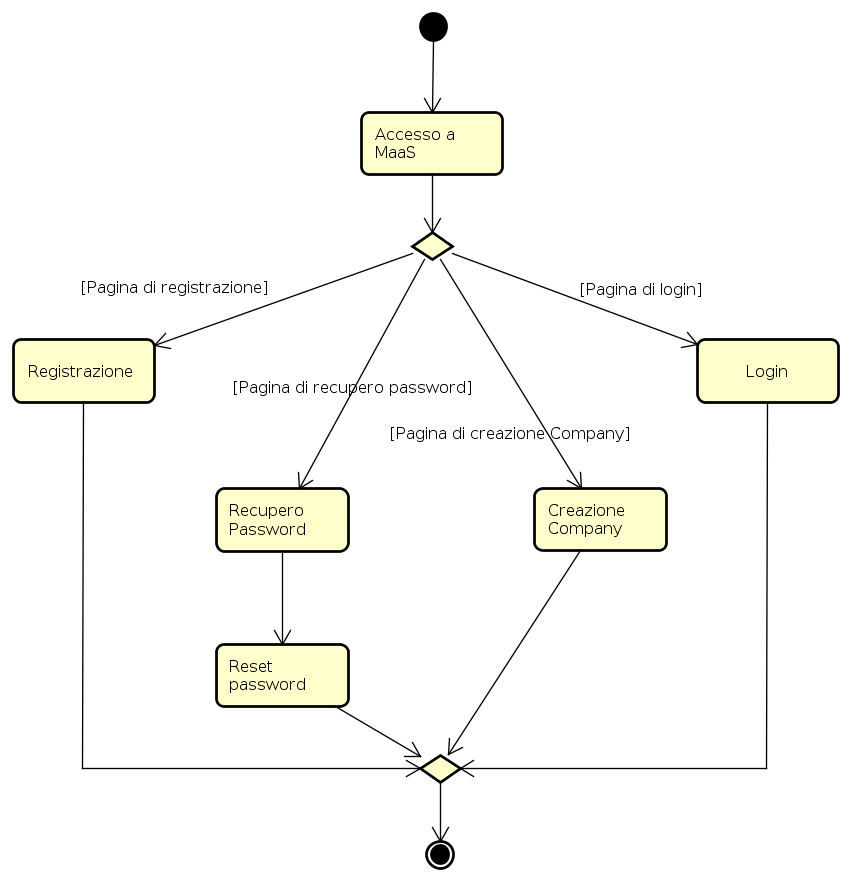
\includegraphics[height=12cm]{res/sections/backend/activities/principaliSenzaAuth.png}
\caption{Attività principali per un utente non autenticato}
\end{center}
\end{figure}
Un utente non autenticato, una volta visualizzata la pagina di MaaS, può:
\begin{itemize}
\item registrarsi, a seguito di un invito di un owner di una company;
\item effettuare il login;
\item eseguire la procedura di recupero password;
\item creare una nuova Company. L'utente verrà registrato come owner della company appena creata.
\end{itemize}
\subsubsection{Registrazione}
\begin{figure}[H]
\begin{center}
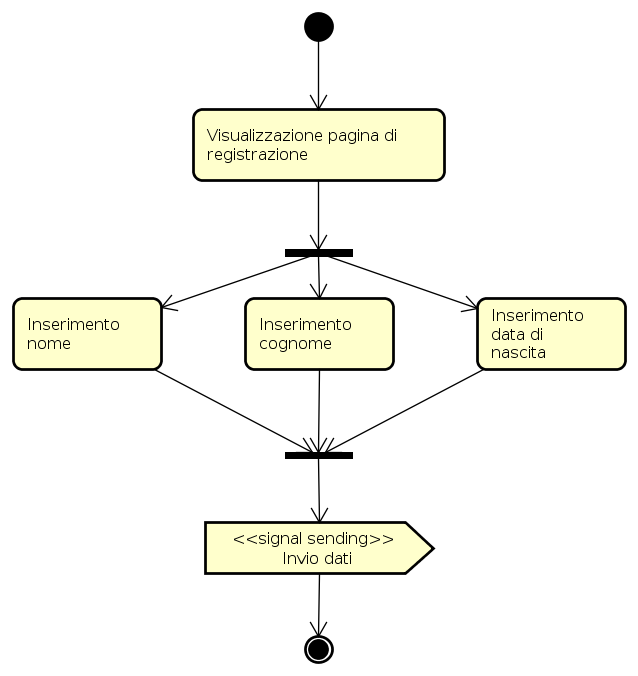
\includegraphics[height=12cm]{res/sections/backend/activities/registrazione.png}
\caption{Registrazione a MaaS}
\end{center}
\end{figure}
L'utente si trova nella pagina di registrazione a MaaS. Indirizzo email e password sono già stati impostati, e potrenno essere modificati dopo il completamento della procedura di registrazione; viene richiesto l'inserimento di tre campi base per il profilo di un utente: nome, cognome e data di nascita.
\subsubsection{Login}
\begin{figure}[H]
\begin{center}
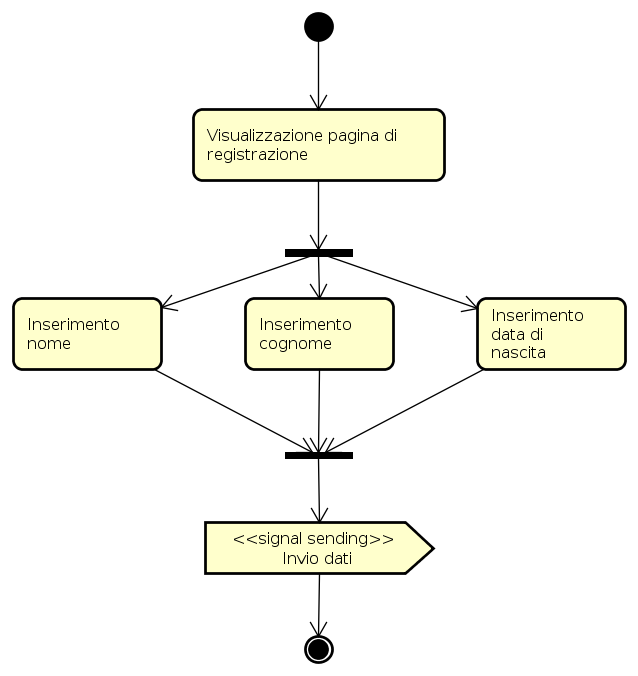
\includegraphics[height=12cm]{res/sections/backend/activities/registrazione.png}
\caption{Login}
\end{center}
\end{figure}
L'utente non autenticato deve inserire, in due caselle di testo, le proprie credenziali di accesso, username e password, per poter accedere a MaaS. Se le credenziali risultano valide l'utente veràà reindirizzato alla pagina contenente la propria dashboard, altrimenti verrà mostrato un messaggio di errore.
\subsubsection{Recupero password}
\begin{figure}[H]
\begin{center}
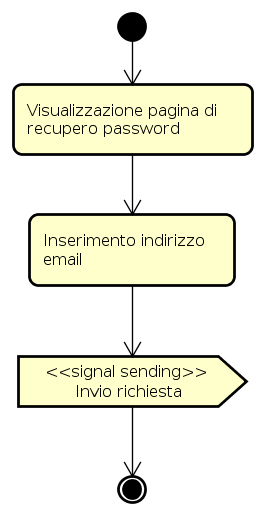
\includegraphics[height=12cm]{res/sections/backend/activities/recuperoPassword.png}
\caption{Recupero password}
\end{center}
\end{figure}
L'utente non autenticato deve inserire, in una casella di testo, l'indirizzo email al quale sarà inviato il codice segreto da utilizzare nella procedura di reset della password.
\subsubsection{Reset password}
\begin{figure}[H]
\begin{center}
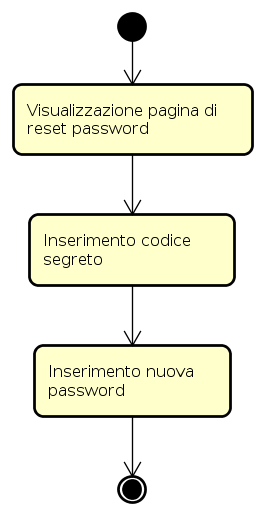
\includegraphics[height=12cm]{res/sections/backend/activities/resetPassword.png}
\caption{Reset password}
\end{center}
\end{figure}
L'utente non autenticato deve inserire, in una casella di testo, il codice segreto che ha ricevuto tramite email necessario a eseguire il reset della password. Se il codice è verificato, l'utente non autenticato potrà inserire una nuova password, che verrà memorizzata al posto della vecchia.
\subsubsection{Creazione company}
\begin{figure}[H]
\begin{center}
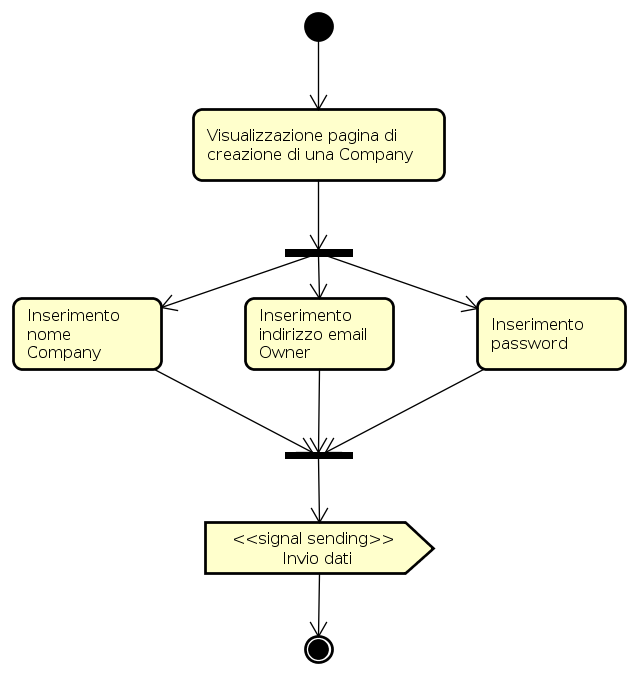
\includegraphics[height=12cm]{res/sections/backend/activities/creazioneCompany.png}
\caption{Creazione company}
\end{center}
\end{figure}
L'utente non autenticato che crea una company viene registrato come suo owner. È pertanto necessario fornire, durante la procedura di creazione, l'indirizzo email e la password dell'utente, oltre che il nome della company stessa.
\subsection{Utente autenticato}
%todo
\subsection{Editor}
%todo
\subsection{Super Admin}
\begin{figure}[H]
\begin{center}
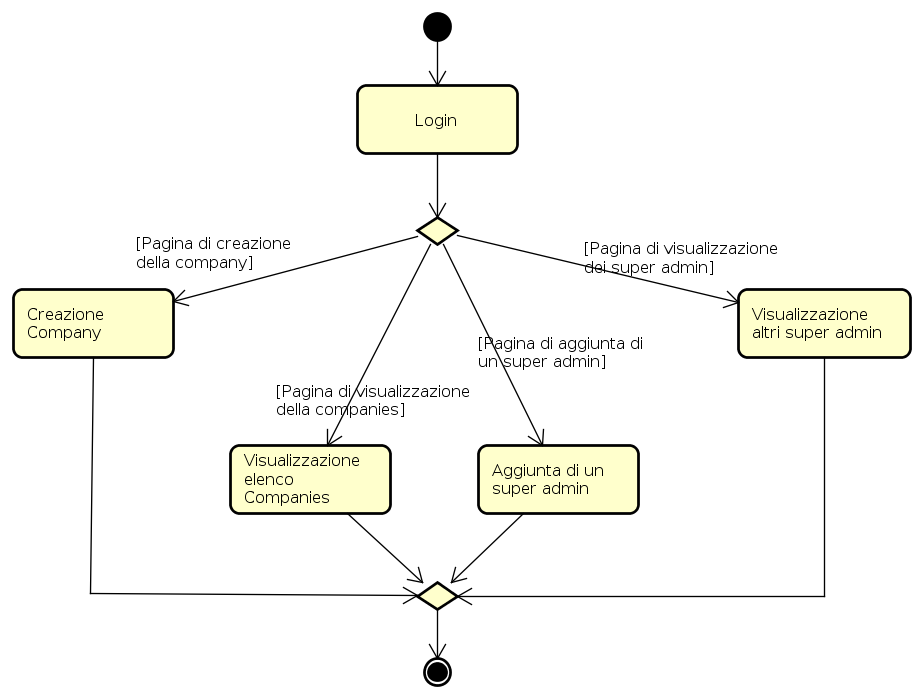
\includegraphics[height=12cm]{res/sections/backend/activities/principaliSuperAdmin.png}
\caption{Attività principali per il super admin}
\end{center}
\end{figure}
Dopo aver effettuato il login, il super admin può:
\begin{itemize}
\item creare una company;
\item visualizzare l'elenco delle company registrate a MaaS;
\item aggiungere un altro super admin;
\item visualizzare i dettagli sugli altri super admin.
\end{itemize}
\subsubsection{Creazione company}
\begin{figure}[H]
\begin{center}
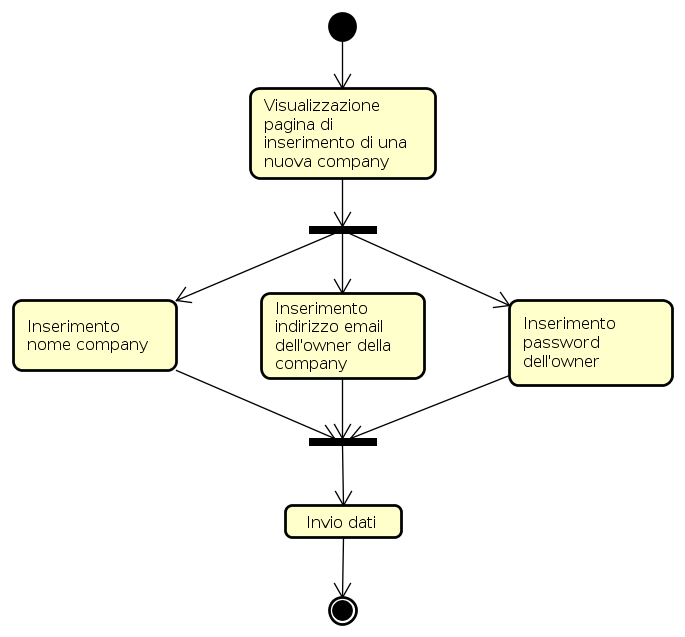
\includegraphics[height=12cm]{res/sections/backend/activities/creazioneCompanySA.png}
\caption{Creazione company}
\end{center}
\end{figure}
Il super admin che crea una company deve fornire i dati dell'utente che verrà registrato come owner. È pertanto necessario fornire, durante la procedura di creazione, l'indirizzo email e la password del nuovo utente, oltre che il nome della company stessa.
\subsubsection{Visualizzazione elenco companies}
\begin{figure}[H]
\begin{center}
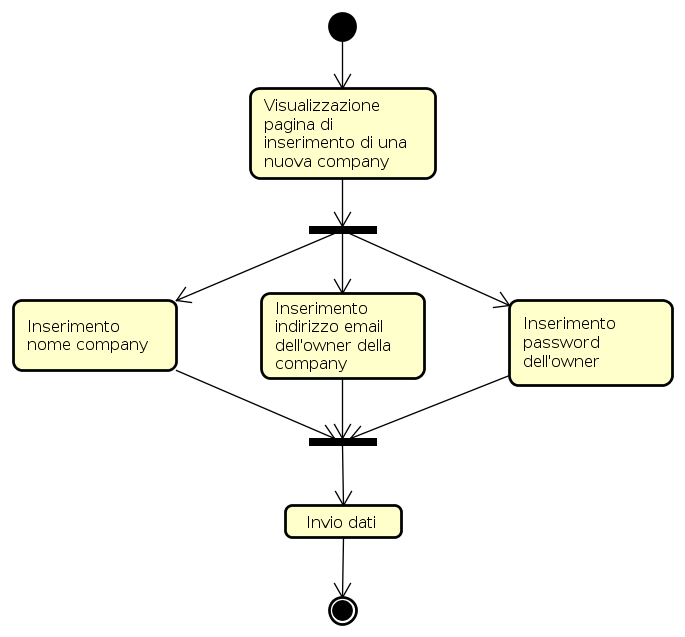
\includegraphics[height=12cm]{res/sections/backend/activities/creazioneCompanySA.png}
\caption{Visualizzazione elenco companies}
\end{center}
\end{figure}
Il super admin può visualizzare tutte le company presenti in MaaS, ed eseguire varie operazioni su di esse:
\begin{itemize}
\item modificare i dati della company;
\item aggiungere un utente;
\item visualizzarne gli utenti.
\end{itemize}
\paragraph{Modifica company} \mbox{} \\
\begin{figure}[H]
\begin{center}
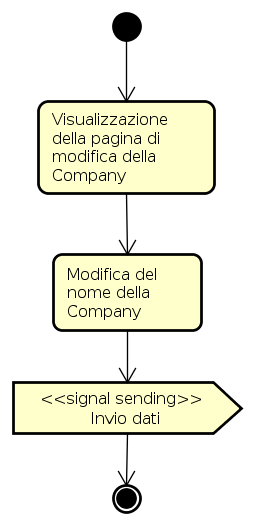
\includegraphics[height=12cm]{res/sections/backend/activities/modificaCompanySA.png}
\caption{Modifica dei dati di una company}
\end{center}
\end{figure}
Il super admin può modificare il nome di una company inserendo il nuovo nome in una casella di testo ed inviando la richiesta di aggiornamento tramite un pulsante presente sulla pagina.
\paragraph{Aggiunta utente} \mbox{} \\
\begin{figure}[H]
\begin{center}
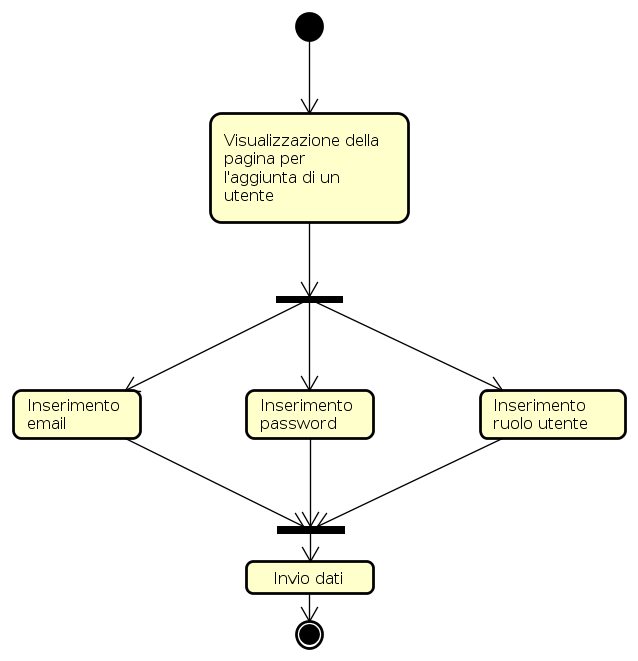
\includegraphics[height=12cm]{res/sections/backend/activities/aggiuntaUtenteSA.png}
\caption{Aggiunta di un utente alla company}
\end{center}
\end{figure}
Il super admin può aggiungere un utente alla company selezionata inserendone indirizzo email, password e ruolo. 
\paragraph{Visualizzazione utenti della company} \mbox{} \\
\begin{figure}[H]
\begin{center}
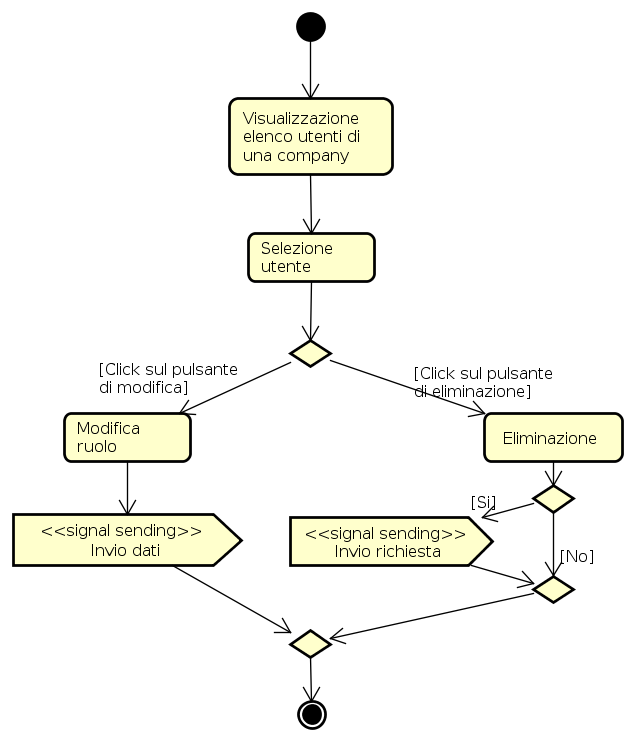
\includegraphics[height=12cm]{res/sections/backend/activities/operazioniUtentiSA.png}
\caption{Visualizzazione utenti della company}
\end{center}
\end{figure}
Una volta visualizato l'elenco degli utenti iscritti alla comapny, il super admin può modificare il ruolo di un utente o di rimuoverlo. Nel secondo caso è richiesta una conferma, per evitare eliminazioni accidentali.
\subsubsection{Aggiunta di un super admin}
\begin{figure}[H]
\begin{center}
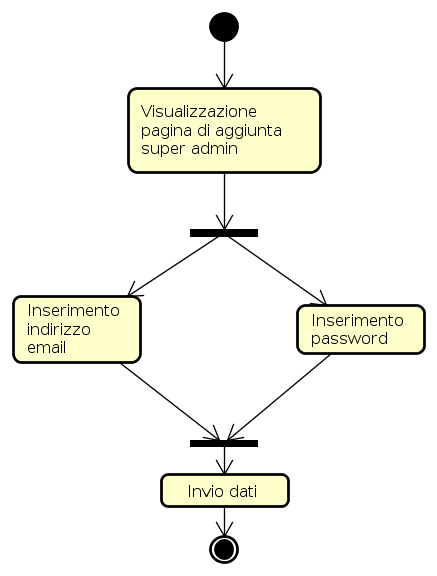
\includegraphics[height=12cm]{res/sections/backend/activities/aggiuntaSuperAdminSA.png}
\caption{Aggiunta super admin}
\end{center}
\end{figure}
Il super admin può visualizzare tutte le company presenti in MaaS, ed eseguire varie Il super admin può inserire un altro super admin all'intero di MaaS, per farlo è necessario fornirne indirizzo email e password, ed inviare i dati attraverso un apposito pulsante.
\subsubsection{Visualizzazione dettagli di un super admin}
\begin{figure}[H]
\begin{center}
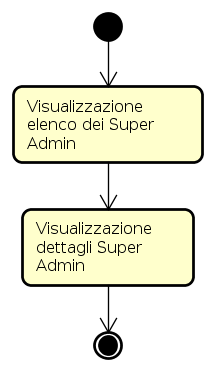
\includegraphics[height=12cm]{res/sections/backend/activities/visualizzazioneDettagliSuperAdminSA.png}
\caption{Visualizzazione altri super admins}
\end{center}
\end{figure}
Il super admin può visualizzare i dettagli sugli altri super admin a partire dalla pagina di elenco dei super admin presenti in MaaS. Per fare questo è sufficiente fare click sul super admin del quale si vogliono visualizzare i dettagli.